% Beispiel für Bild mit Fußnote
\begin{figure}[htb]
 \centering
 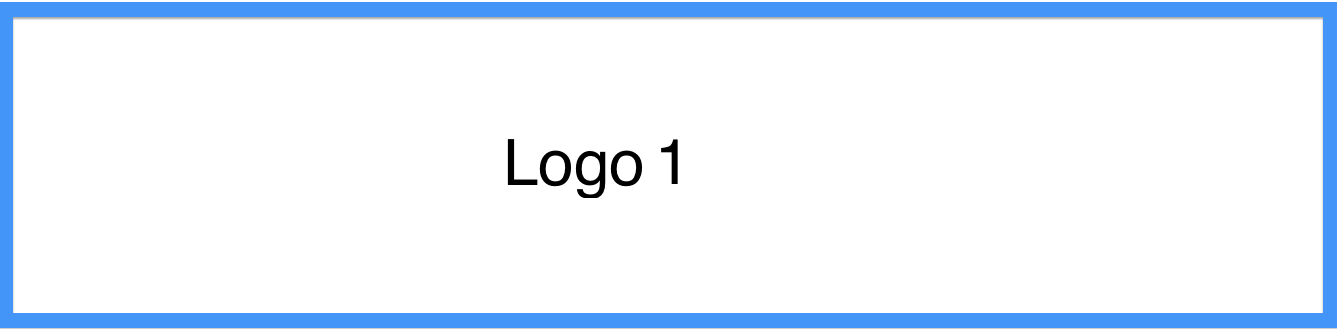
\includegraphics[width=0.4\textwidth,angle=45]{abb/logo1}
 \caption[Beispiel einer Bildbeschreibung]{Beispiel einer Bildbeschreibung\footnotemark}
\label{fig:beispiel1}
\end{figure}
\footnotetext{Bildquelle: Beispielquelle}

% Beispiel für Bildintegration
\begin{figure}[htb]
 \centering
 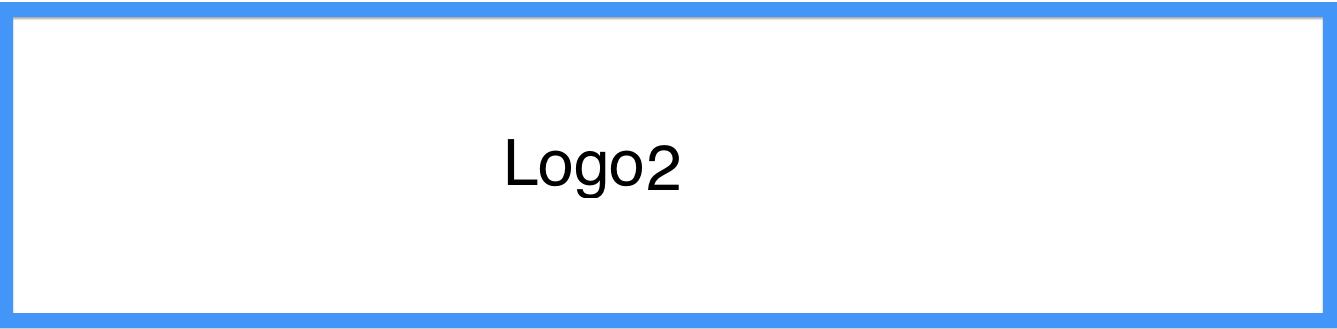
\includegraphics[width=0.3\textwidth,angle=0]{abb/logo2}
 \caption[Beschreibung]{Beschreibung}
\label{fig:Beschreibung}
\end{figure}

% Beispiel: Referenz auf Abbildung
Abbildung~\ref{fig:Beschreibung} [S.\pageref{fig:Beschreibung}]

% Beispiel: Tabelle 
\begin{center}
  \begin{tabular}{ | l | c | }
    \hline
    Überschrift 1 & Überschrift 2 \\ \hline \hline
    Info 1 & Info 2 \\ \hline
    Info 3 & Info 4 \\
    \hline
  \end{tabular}
\end{center}


% Beispiel für Quellcode Listings
\lstset{language=xml}
\begin{lstlisting}[frame=htrbl, caption={Die Datei {\tt data-config.xml} dient als Beispiel für XML Quellcode}, label={lst:dataconfigxml}]
<dataConfig>
  <dataSource type="JdbcDataSource" 
              driver="com.mysql.jdbc.Driver"
              url="jdbc:mysql://localhost/bms_db"
              user="root" 
              password=""/>
  <document>
    <entity name="id"
        query="select id, htmlBody, sentDate, sentFrom, subject, textBody
        from mail">
    <field column="id" name="id"/>
    <field column="htmlBody" name="text"/>
    <field column="sentDate" name="sentDate"/>
    <field column="sentFrom" name="sentFrom"/>
    <field column="subject"  name="subject"/>
    <field column="textBody" name="text"/>
    </entity>
  </document>
</dataConfig>
\end{lstlisting}

\lstset{language=java}
\begin{lstlisting}[frame=htrbl, caption={Das Listing zeigt Java Quellcode}, label={lst:result2}]
/* generate TagCloud */
Cloud cloud = new Cloud();
cloud.setMaxWeight(_maxSizeOfText);
cloud.setMinWeight(_minSizeOfText);
cloud.setTagCase(Case.LOWER);
	    
/* evaluate context and find additional stopwords */
String query = getContextQuery(_context);
List<String> contextStoplist = new ArrayList<String>();
contextStoplist = getStopwordsFromDB(query);
	    
/* append context stoplist */
while(contextStoplist != null && !contextStoplist.isEmpty())
  _stoplist.add(contextStoplist.remove(0));
	    
/* add cloud filters */
if (_stoplist != null) {
  DictionaryFilter df = new DictionaryFilter(_stoplist);
  cloud.addInputFilter(df);
}
/* remove empty tags */
NonNullFilter<Tag> nnf = new NonNullFilter<Tag>();
cloud.addInputFilter(nnf);

/* set minimum tag length */
MinLengthFilter mlf = new MinLengthFilter(_minTagLength);
cloud.addInputFilter(mlf);

/* add taglist to tagcloud */
cloud.addText(_taglist);

/* set number of shown tags */	    
cloud.setMaxTagsToDisplay(_tagsToDisplay);
\end{lstlisting}


% Beispiel für Formeln
Die Zuordnung aller möglichen Werte, welche eine Zufallsvariable annehmen kann nennt man \emph{Verteilungsfunktion} von $X$.

\begin{quotation}
Die Funktion F: $\mathbb{R} \rightarrow$ [0,1] mit $F(t) = P (X \le t)$ heißt Verteilungsfunktion von $X$.\footnote{Konen, vgl.~\cite{wk05}~[S.55]}
\end{quotation}

\begin{quotation}
Für eine stetige Zufallsvariable $X: \Omega \rightarrow \mathbb{R}$ heißt eine integrierbare, nichtnegative reelle Funktion $w: \mathbb{R} \rightarrow \mathbb{R}$ mit $F(x) = P(X \le x) = \int_{-\infty}^{x} w(t)dt$ die \emph{Dichte} oder \emph{Wahrscheinlichkeitsdichte} der Zufallsvariablen $X$.\footnote{Konen, vgl.~\cite{wk05}~[S.56]}
\end{quotation}
